\documentclass[tikz, border=10pt]{standalone}
\usetikzlibrary{calc, positioning, decorations.pathreplacing, arrows.meta}

\tikzset{
  cell/.style={rectangle, draw=gray!40, thick, minimum size=0.7cm, inner sep=0pt},
  rowhl/.style={fill=blue!20, draw=blue!60, thick},
  colhl/.style={fill=orange!25, draw=orange!70, thick},
  reshl/.style={fill=purple!20, draw=purple!60, thick},
  matlabel/.style={font=\Large\bfseries},
}

\begin{document}
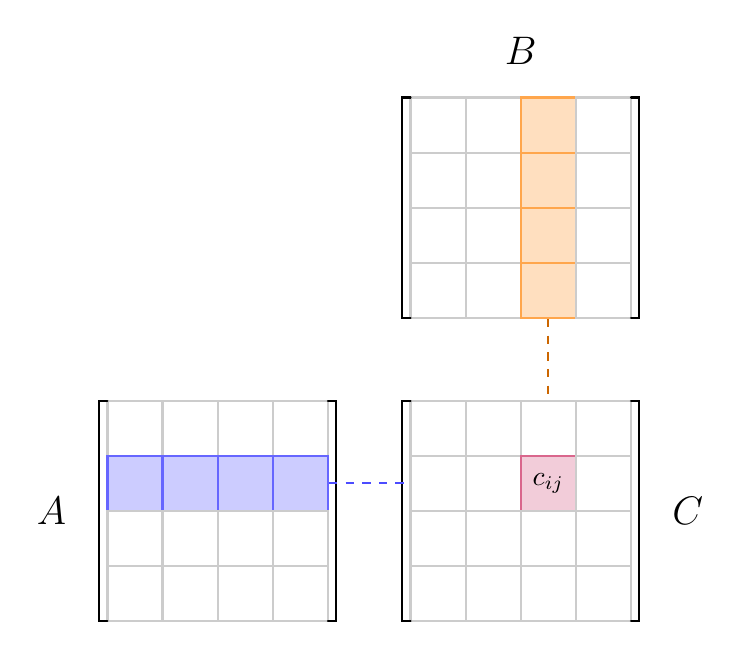
\begin{tikzpicture}[x=0.7cm, y=0.7cm]
  \def\n{4} % Matrix dimension (4x4)

  % --- MATRIX A (Bottom-Left) ---
  \begin{scope}[shift={(0,0)}]
    \node[matlabel, left=0.4cm] at (0, \n/2) {$A$};
    \foreach \r in {1,...,\n} {
      \foreach \c in {1,...,\n} {
        \ifnum\r=2
          \node[cell, rowhl] (A-\r-\c) at (\c-0.5, \n-\r+0.5) {};
        \else
          \node[cell] (A-\r-\c) at (\c-0.5, \n-\r+0.5) {};
        \fi
      }
    }
    \draw[thick, line cap=round] (0, 0) -- (-0.15, 0) -- (-0.15, \n) -- (0, \n);
    \draw[thick, line cap=round] (\n, 0) -- (\n+0.15, 0) -- (\n+0.15, \n) -- (\n, \n);
  \end{scope}

  % --- MATRIX B (Top-Right) ---
  \begin{scope}[shift={(5.5,5.5)}]
    \node[matlabel, above=0.3cm] at (\n/2, \n) {$B$};
    \foreach \r in {1,...,\n} {
      \foreach \c in {1,...,\n} {
        \ifnum\c=3
          \node[cell, colhl] (B-\r-\c) at (\c-0.5, \n-\r+0.5) {};
        \else
          \node[cell] (B-\r-\c) at (\c-0.5, \n-\r+0.5) {};
        \fi
      }
    }
    \draw[thick, line cap=round] (0, 0) -- (-0.15, 0) -- (-0.15, \n) -- (0, \n);
    \draw[thick, line cap=round] (\n, 0) -- (\n+0.15, 0) -- (\n+0.15, \n) -- (\n, \n);
  \end{scope}

  % --- MATRIX C (Bottom-Right) ---
  \begin{scope}[shift={(5.5,0)}]
    \node[matlabel, right=0.4cm] at (\n, \n/2) {$C$};
    \foreach \r in {1,...,\n} {
      \foreach \c in {1,...,\n} {
        \ifnum\r=2
          \ifnum\c=3
            \node[cell, reshl] (C-\r-\c) at (\c-0.5, \n-\r+0.5) {$c_{ij}$};
          \else
            \node[cell] (C-\r-\c) at (\c-0.5, \n-\r+0.5) {};
          \fi
        \else
          \node[cell] (C-\r-\c) at (\c-0.5, \n-\r+0.5) {};
        \fi
      }
    }
    \draw[thick, line cap=round] (0, 0) -- (-0.15, 0) -- (-0.15, \n) -- (0, \n);
    \draw[thick, line cap=round] (\n, 0) -- (\n+0.15, 0) -- (\n+0.15, \n) -- (\n, \n);
  \end{scope}

  % --- PROJECTION LINES ---
  \draw[blue!70, dashed, thick] (A-2-4.east) -- (C-2-1.west);
  \draw[orange!80!black, dashed, thick] (B-4-3.south) -- (C-1-3.north);

\end{tikzpicture}
\end{document}
